\section{Detecting Multiple Objects}
\begin{frame}{}
    \LARGE Object Detection: \textbf{Detecting Multiple Objects}
\end{frame}

\begin{frame}[allowframebreaks]{Multiple Objects}

\begin{figure}
\centering
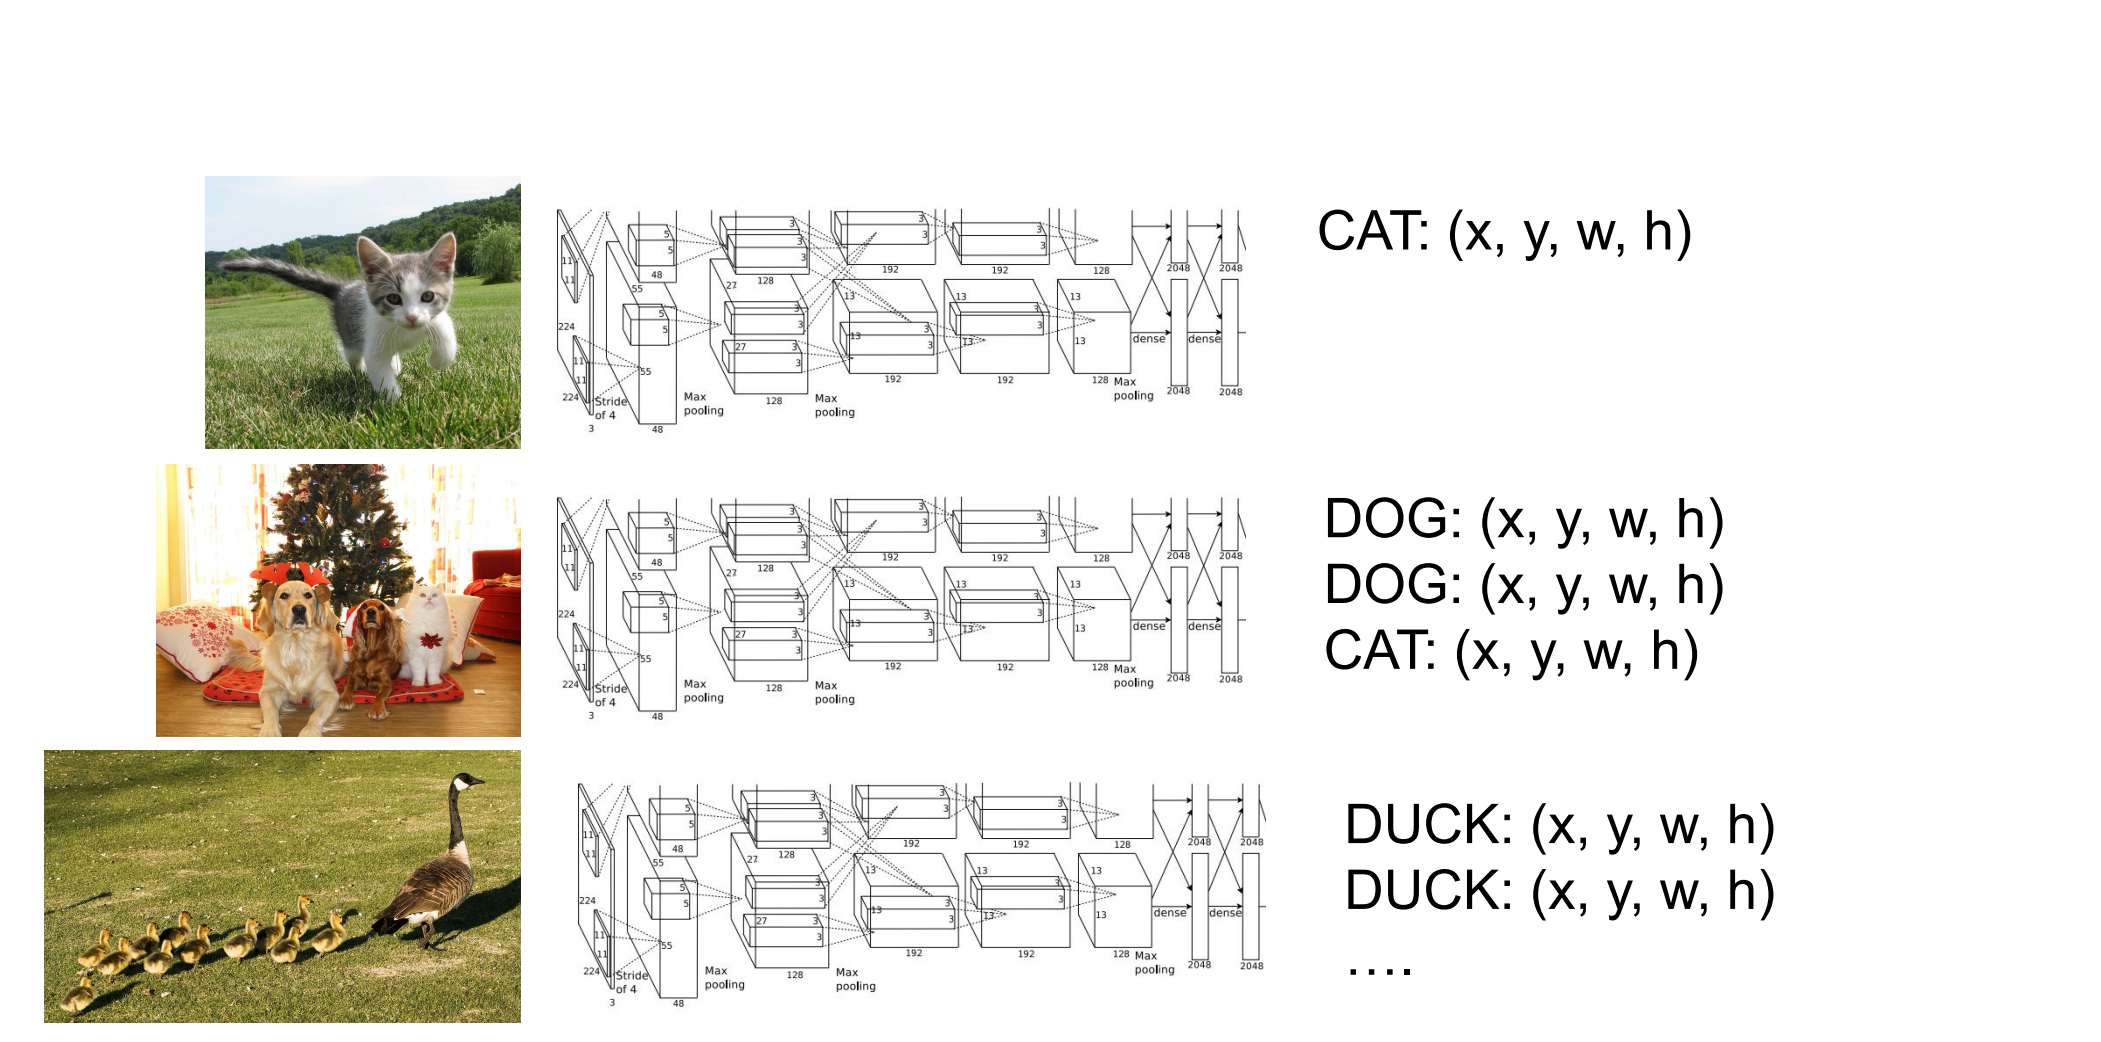
\includegraphics[width=1.0\textwidth,height=0.85\textheight,keepaspectratio]{images/object-detect/object_8.png}
\caption*{\tiny Source: Stanford CS231n (2021), Lecture 15: Detection and Segmentation, slide 41}
\end{figure}

\framebreak

\begin{figure}
\centering
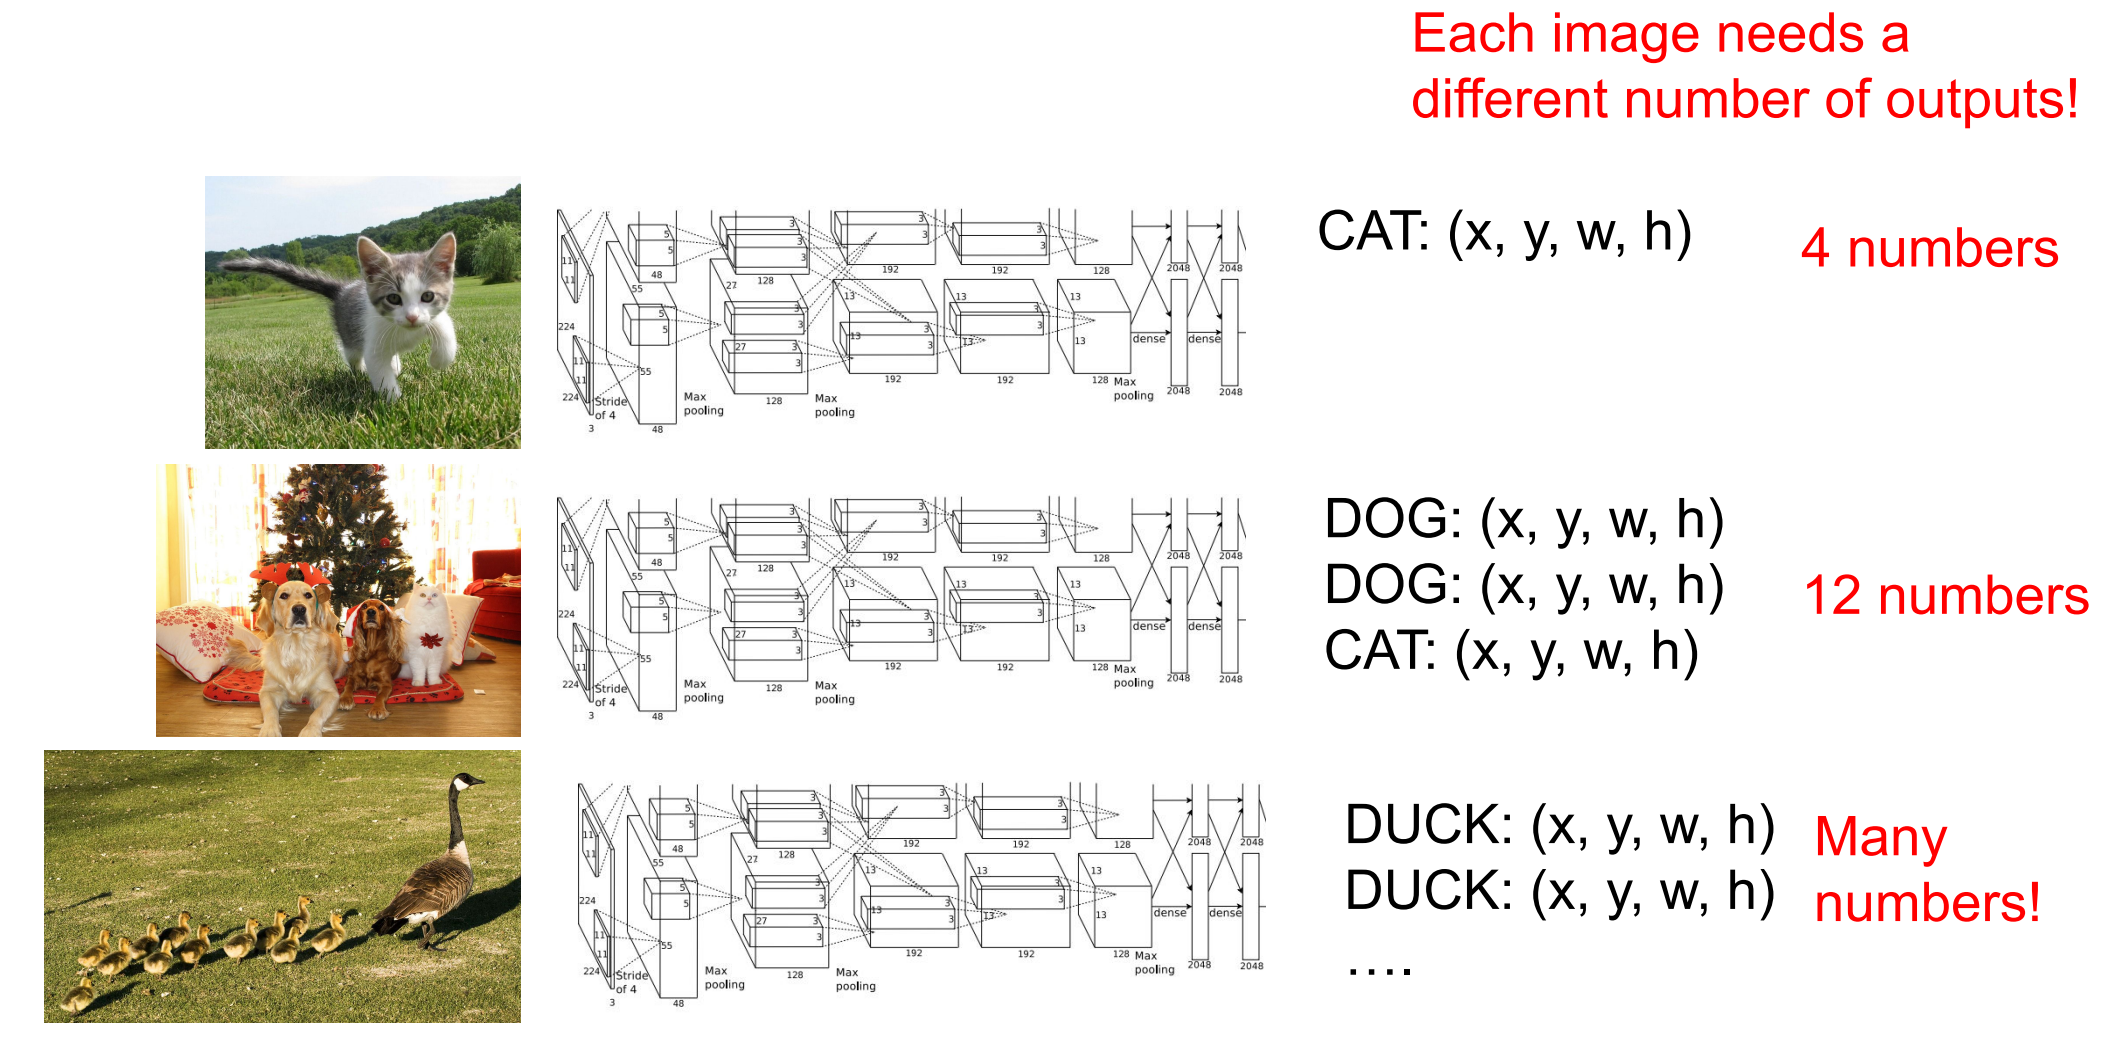
\includegraphics[width=1.0\textwidth,height=0.85\textheight,keepaspectratio]{images/object-detect/object_9.png}
\caption*{\tiny Source: Stanford CS231n (2021), Lecture 15: Detection and Segmentation, slide 42}
\end{figure}

\end{frame}

\subsection{Sliding Window}
\begin{frame}{}
    \LARGE Object Detection: \textbf{Detecting Multiple Objects: Sliding Window}
\end{frame}

\begin{frame}[allowframebreaks]{Detecting Multiple Objects: Sliding Window}

\begin{figure}
\centering
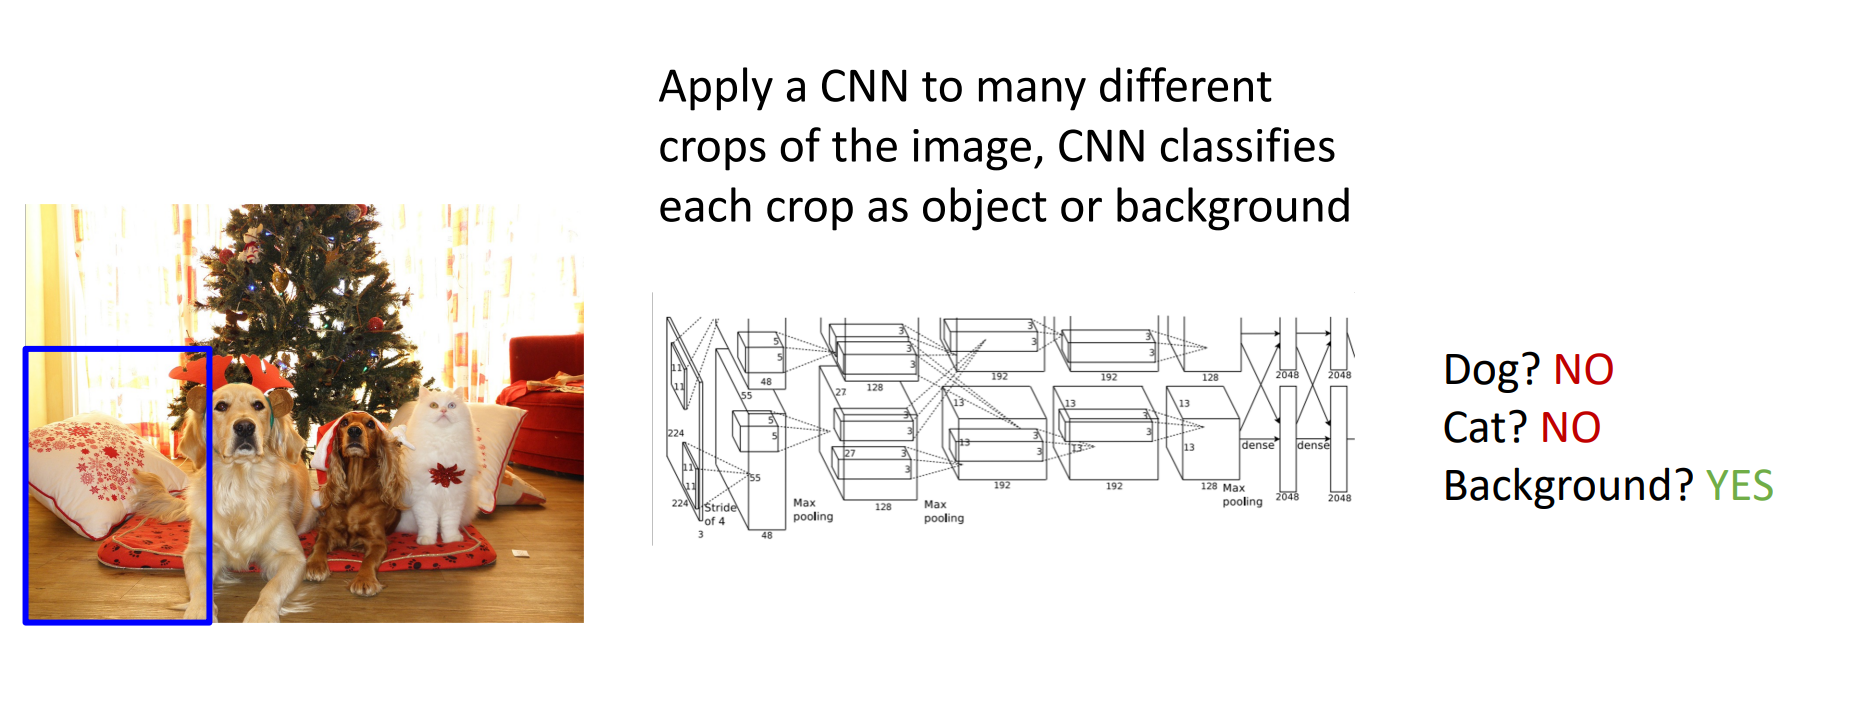
\includegraphics[width=1.0\textwidth,height=0.85\textheight,keepaspectratio]{images/object-detect/object_10.png}
\caption*{\tiny Source: UMich EECS 498 (2022), Lecture 13: Object Detection, slide 52}
\end{figure}

\framebreak

\begin{figure}
\centering
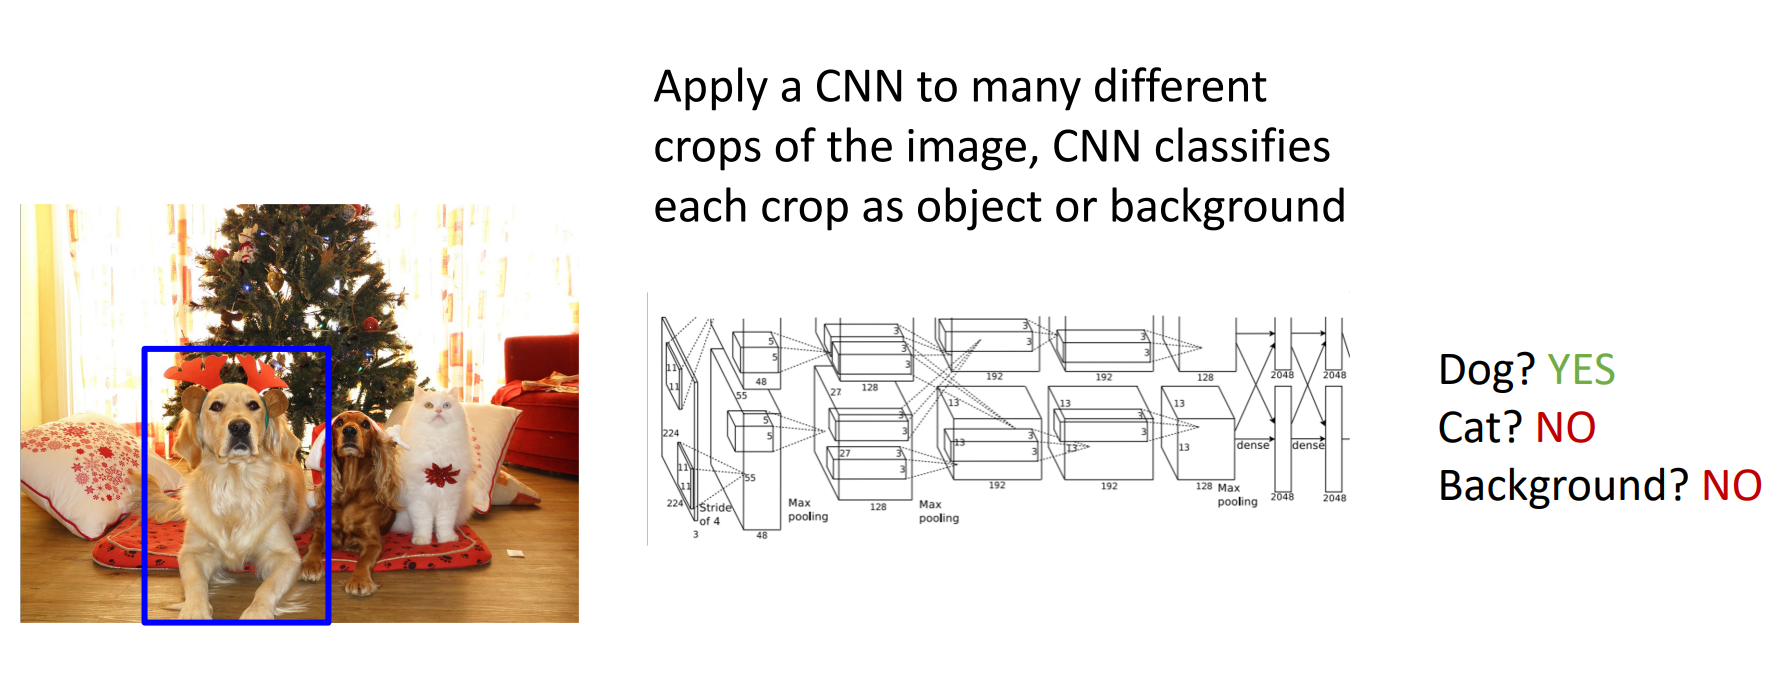
\includegraphics[width=1.0\textwidth,height=0.85\textheight,keepaspectratio]{images/object-detect/object_11.png}
\caption*{\tiny Source: UMich EECS 498 (2022), Lecture 13: Object Detection, slide 53}
\end{figure}

\framebreak

\begin{figure}
\centering
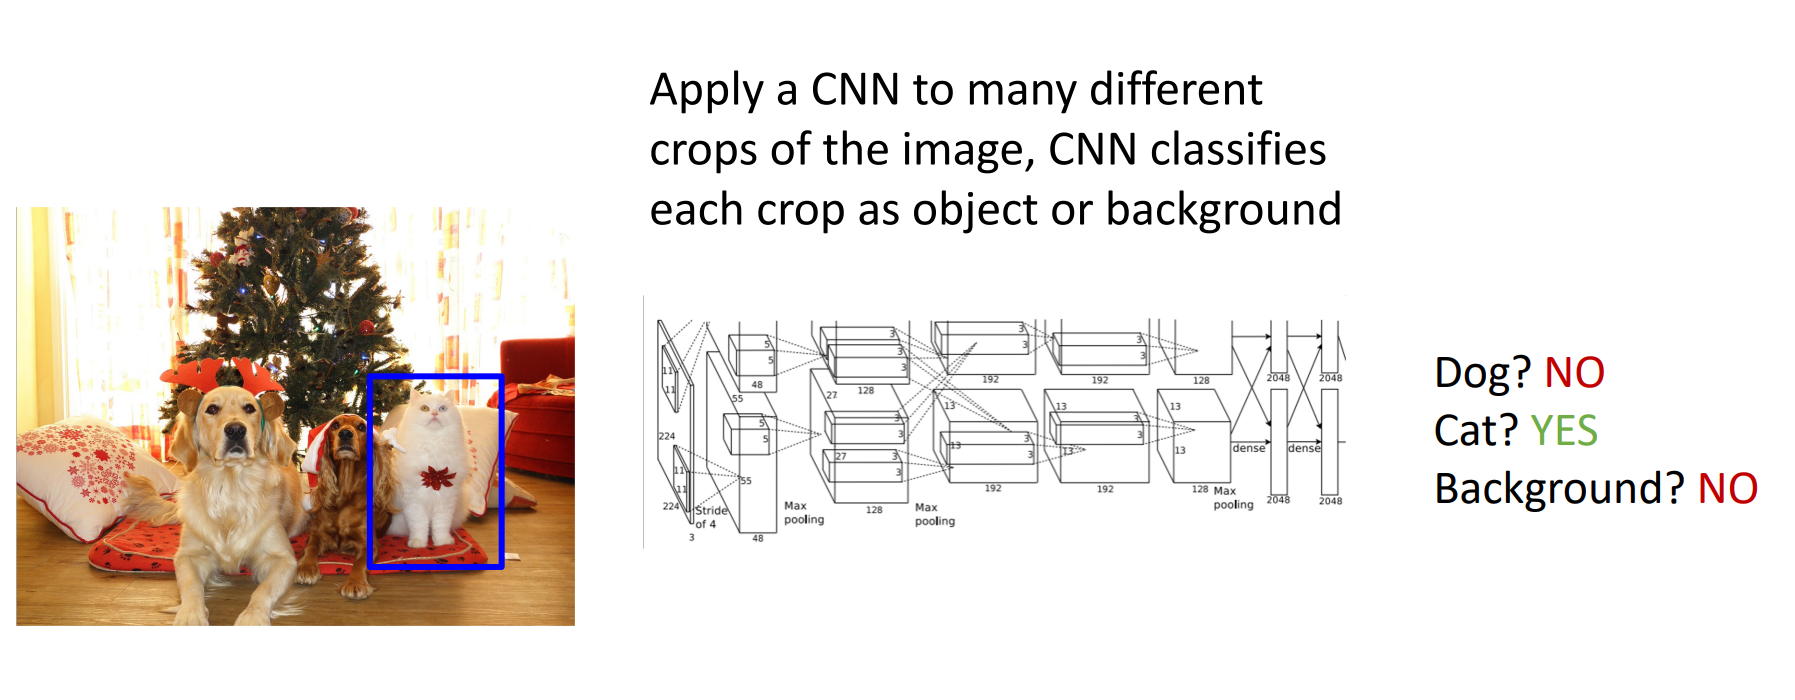
\includegraphics[width=1.0\textwidth,height=0.85\textheight,keepaspectratio]{images/object-detect/object_12.png}
\caption*{\tiny Source: UMich EECS 498 (2022), Lecture 13: Object Detection, slide 55}
\end{figure}

\framebreak

\begin{figure}
\centering
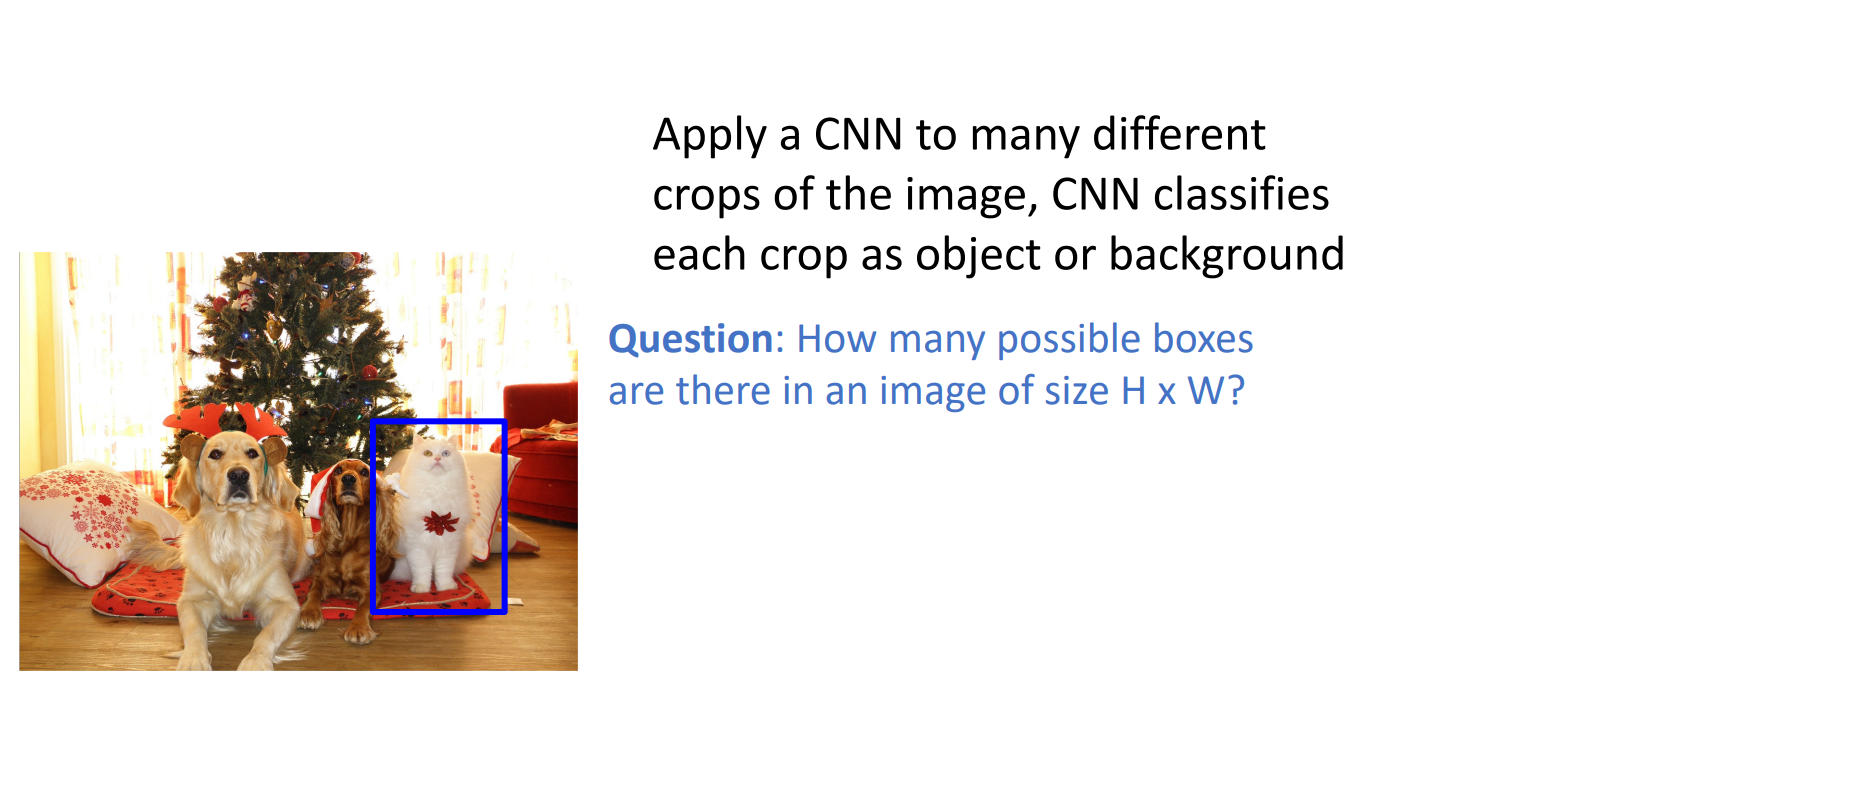
\includegraphics[width=1.0\textwidth,height=0.85\textheight,keepaspectratio]{images/object-detect/object_13.png}
\caption*{\tiny Source: UMich EECS 498 (2022), Lecture 13: Object Detection, slide 56}
\end{figure}

\framebreak

\begin{figure}
\centering
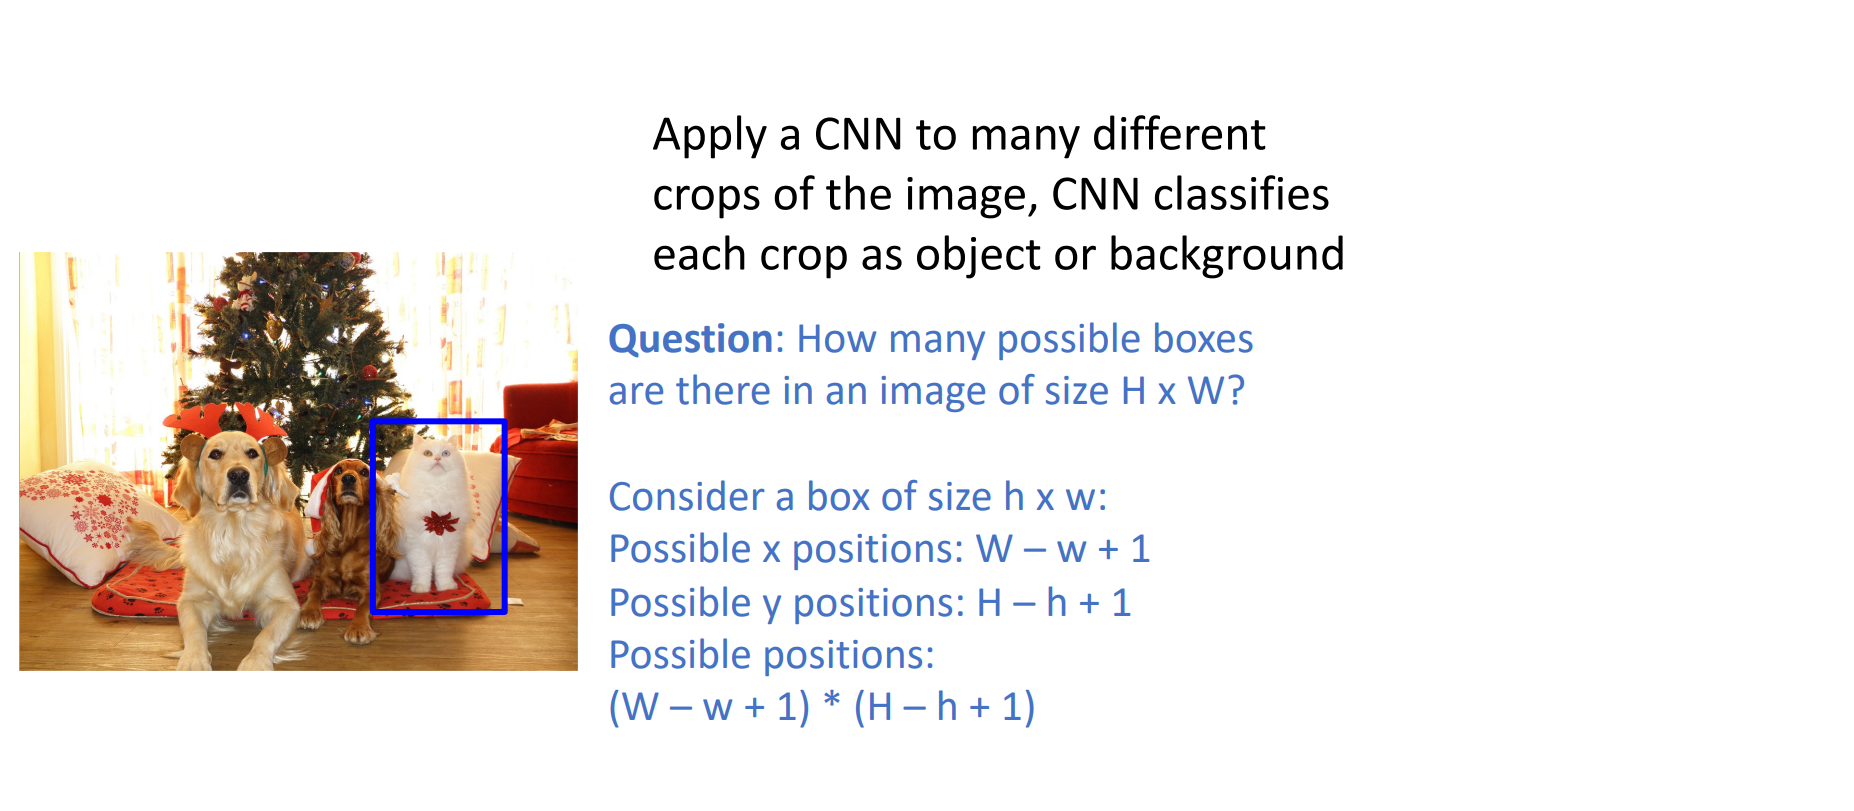
\includegraphics[width=1.0\textwidth,height=0.85\textheight,keepaspectratio]{images/object-detect/object_14.png}
\caption*{\tiny Source: UMich EECS 498 (2022), Lecture 13: Object Detection, slide 57}
\end{figure}

\framebreak

\begin{figure}
\centering
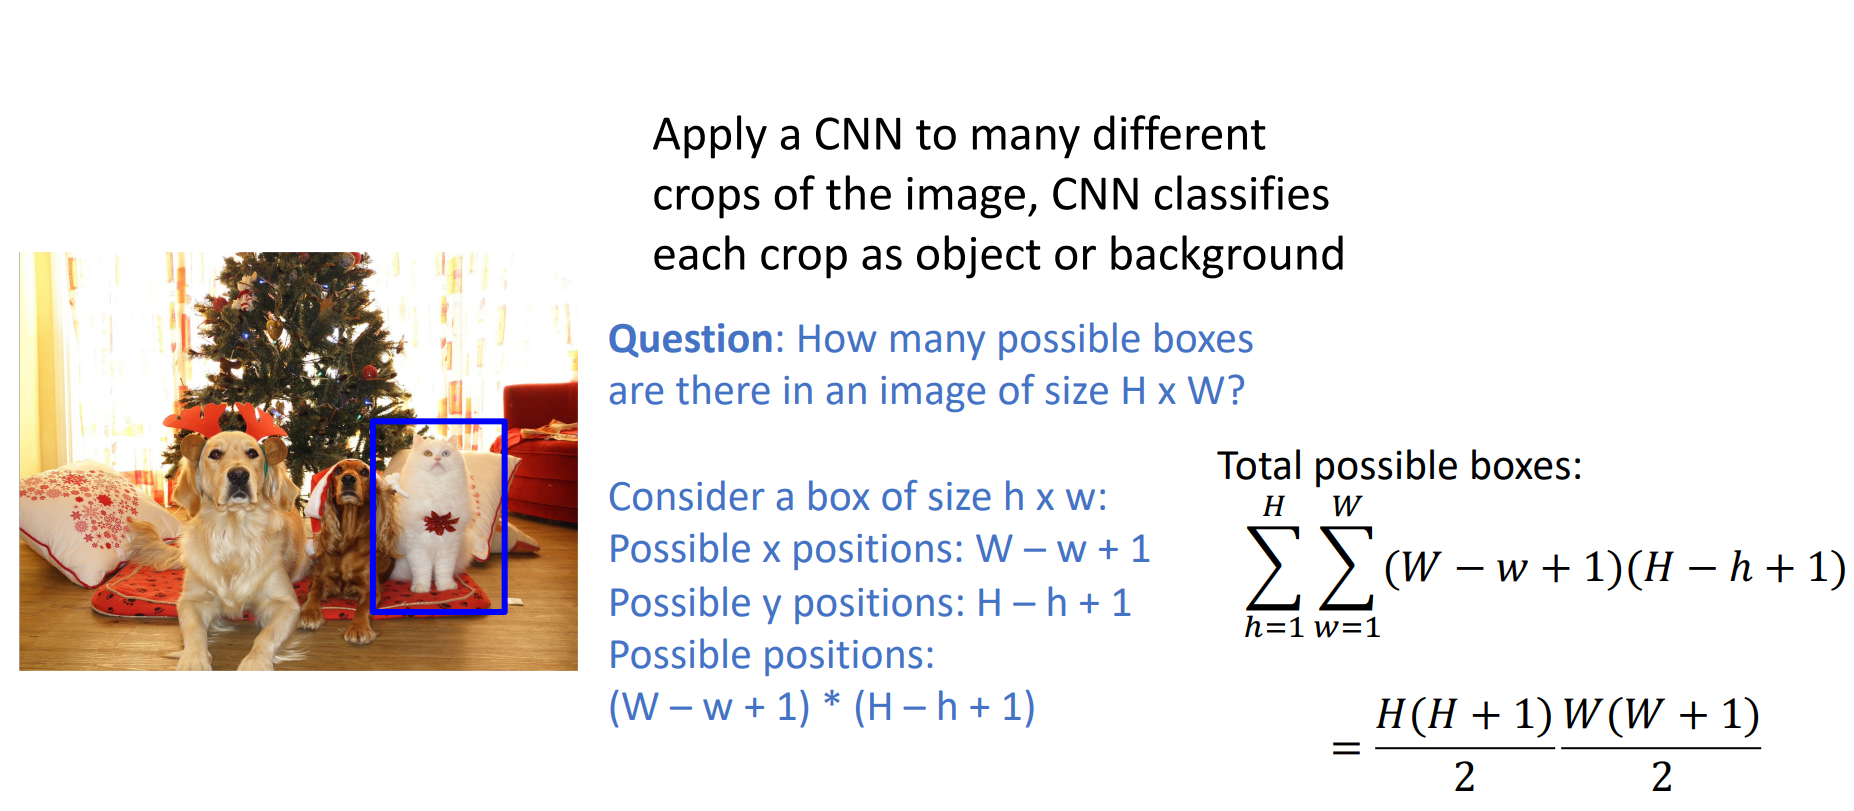
\includegraphics[width=1.0\textwidth,height=0.85\textheight,keepaspectratio]{images/object-detect/object_15.png}
\caption*{\tiny Source: UMich EECS 498 (2022), Lecture 13: Object Detection, slide 58}
\end{figure}

\framebreak

\begin{figure}
\centering
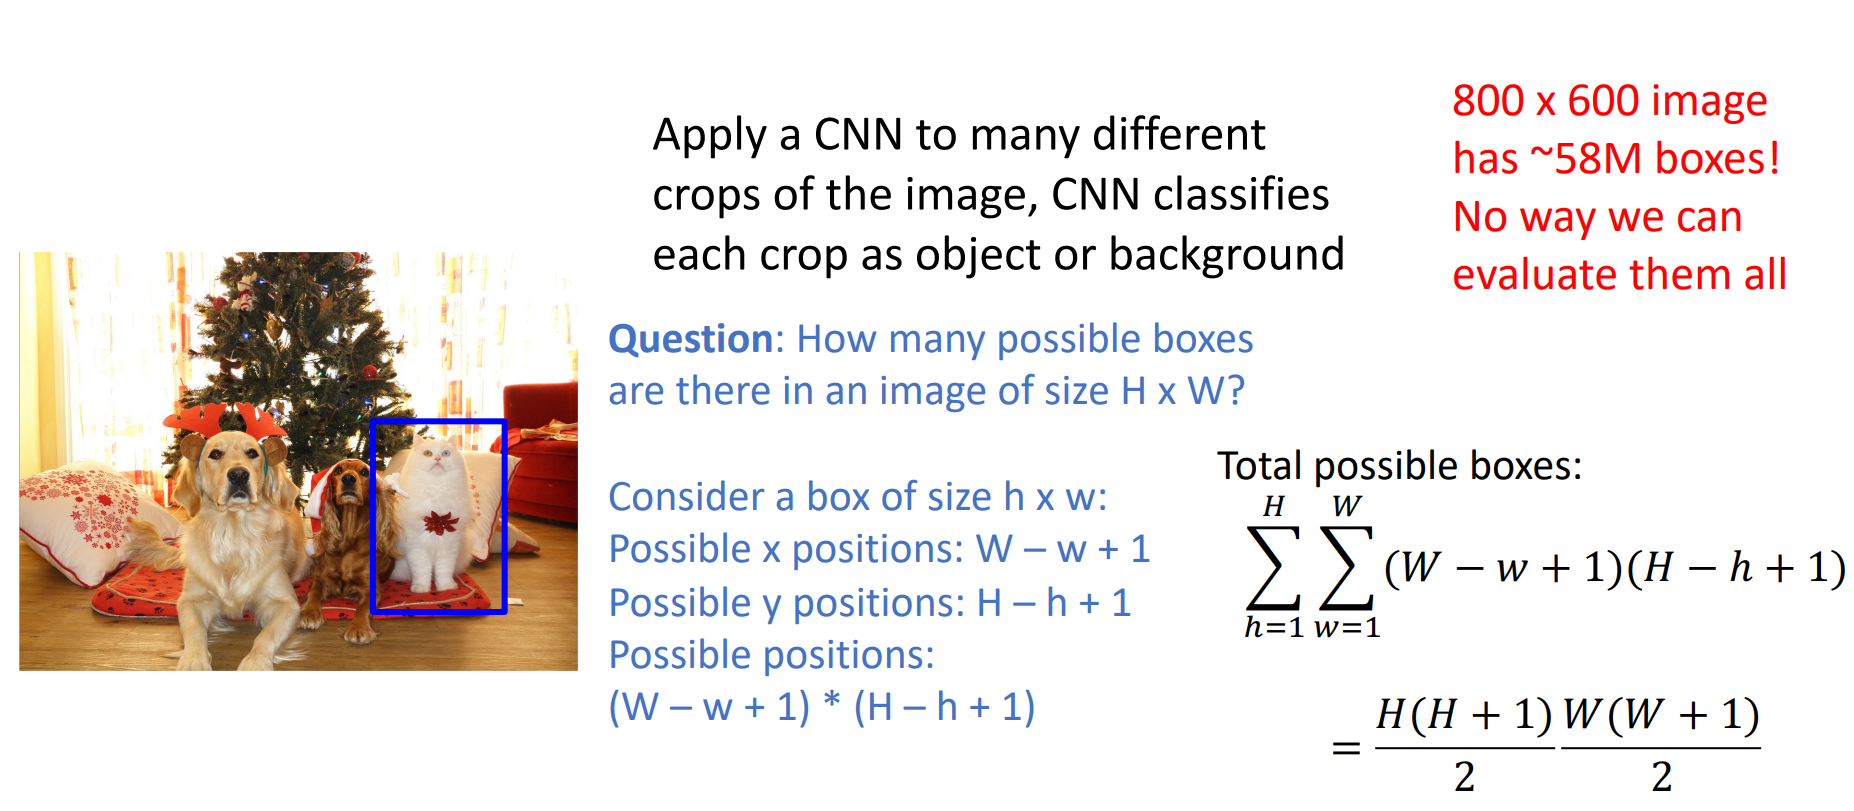
\includegraphics[width=1.0\textwidth,height=0.85\textheight,keepaspectratio]{images/object-detect/object_16.png}
\caption*{\tiny Source: UMich EECS 498 (2022), Lecture 13: Object Detection, slide 59}
\end{figure}
\footnotetext{Correction: the figure's own formula $\tfrac{H(H+1)}{2}\cdot\tfrac{W(W+1)}{2}$ gives $\approx 5.8\times10^{10}$ boxes, i.e.\ about 58 \emph{billion}, not 58 million.}

\end{frame}